\newcommand{\posterPolarLosses}[1]{

\setlength{\frameWidth}{#1}
\setlength{\unitlength}{0.02\frameWidth}
\psset{unit=\unitlength}

\rput[lb](0,15){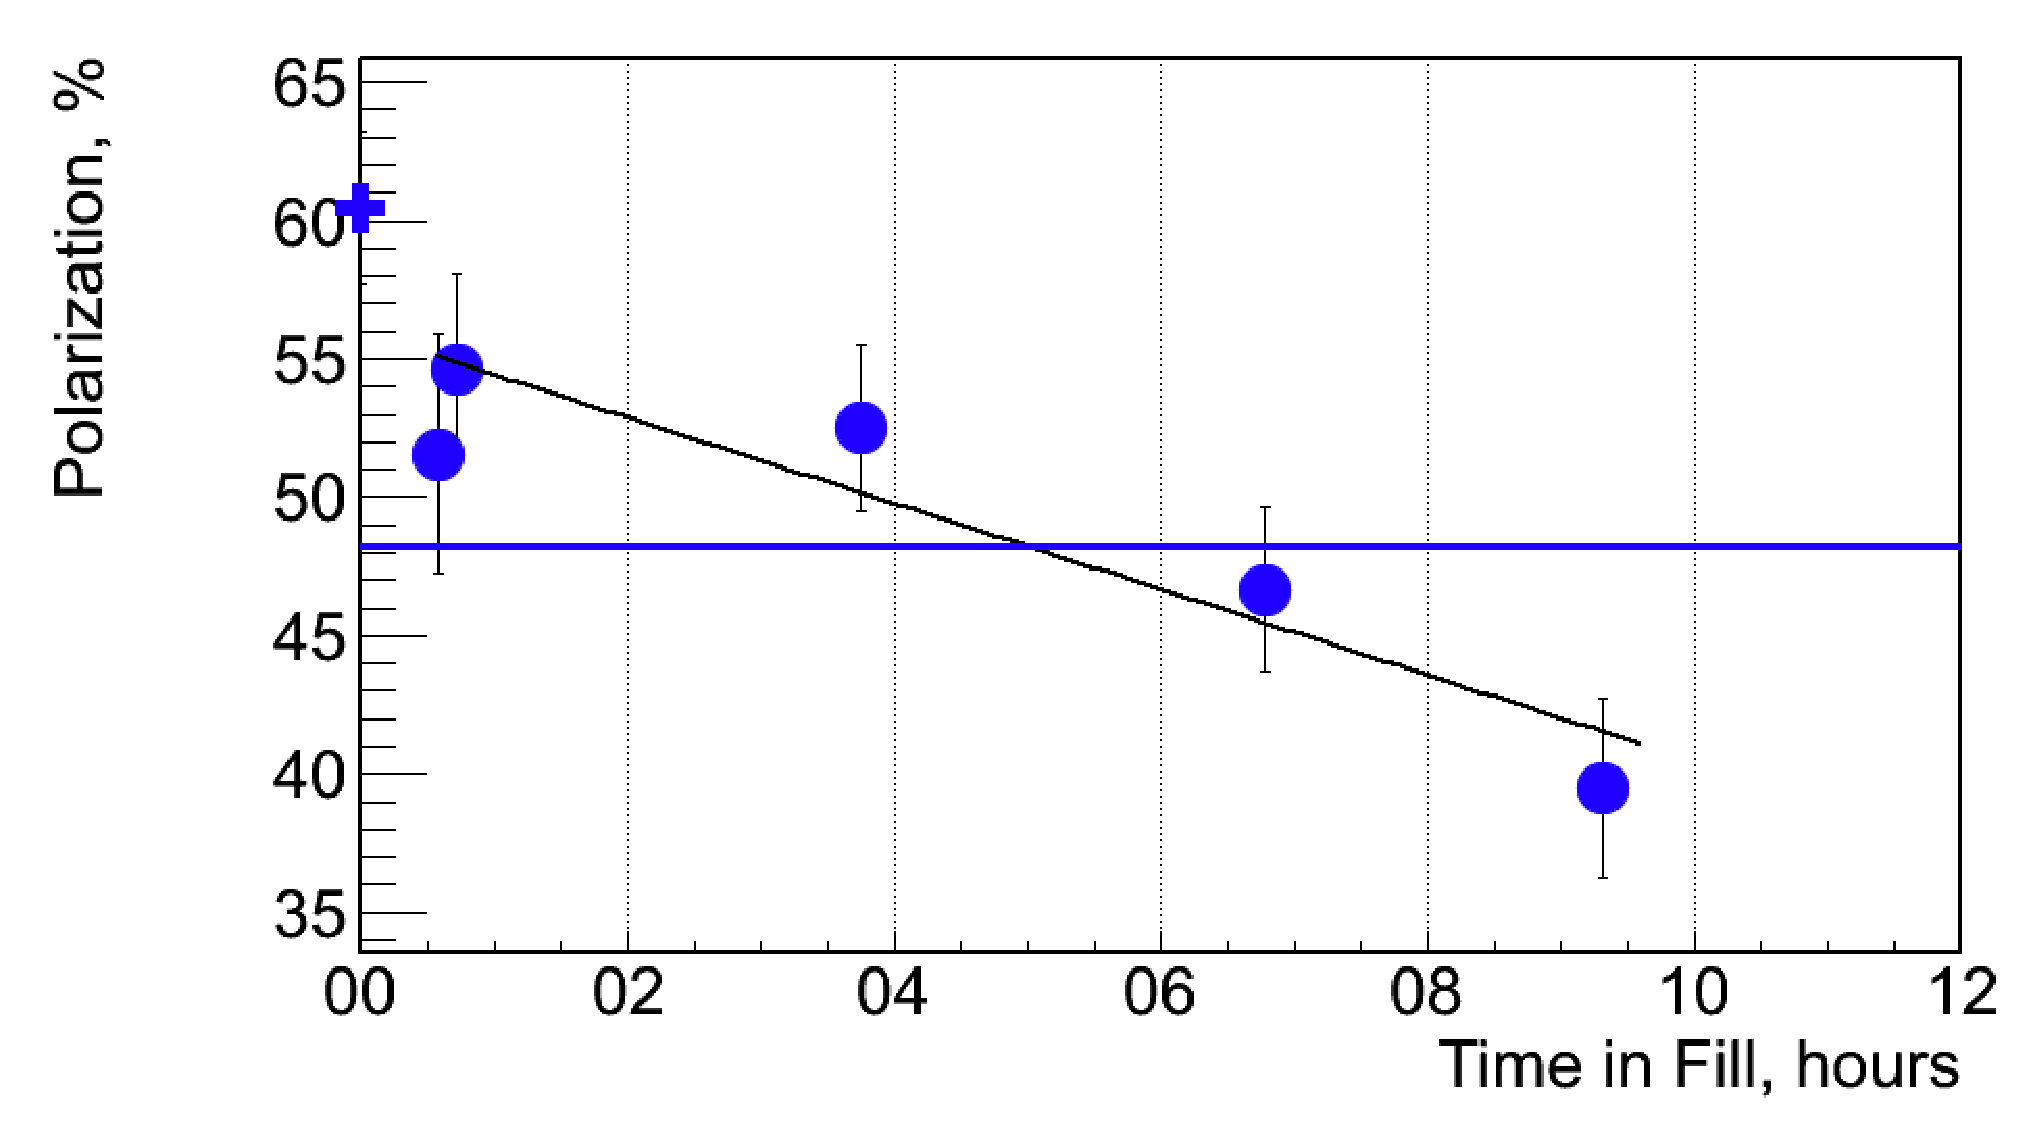
\includegraphics[width=28\unitlength]{graphics/c_hPolarVsFillTime_16650_B1U_crop}}
\rput[lt](0,15){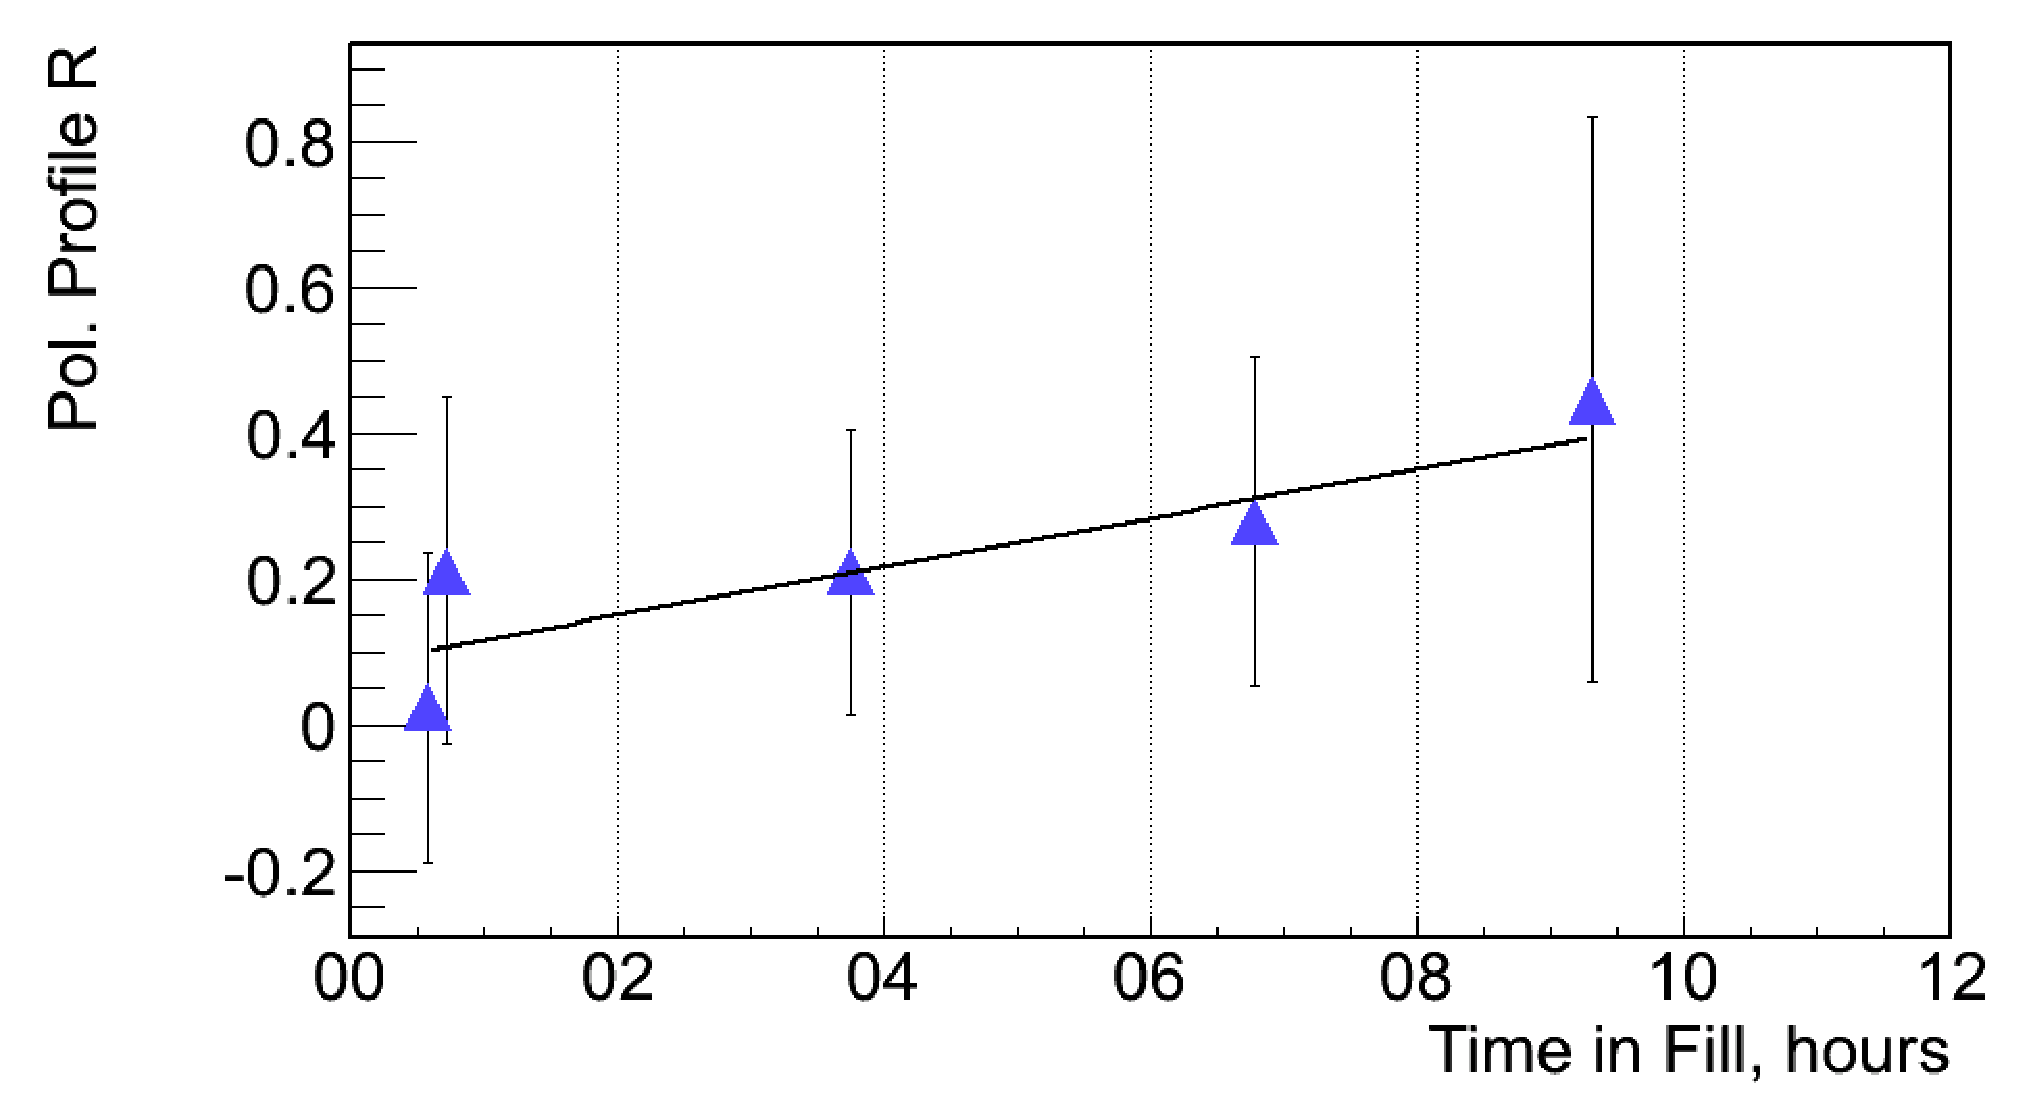
\includegraphics[width=28\unitlength]{graphics/c_hRVsFillTime_16650_B1U_crop}}

\rput[lb](10,28){ \rnode{from}{\psframebox{\small At injection energy} } }
\rput(5,28){ \pnode{to} }
\ncline{->}{from}{to}

\rput[lb](9,18){ \rnode{from}{\psframebox{\small At full energy} } }
\rput(6.5,24){ \pnode{to} }
\ncline{->}{from}{to}
\rput(12,23){ \pnode{to} }
\ncline{->}{from}{to}
\rput(17,21.5){ \pnode{to} }
\ncline{->}{from}{to}
\rput(21,19){ \pnode{to} }
\ncline{->}{from}{to}

\rput[lt](30,24) {%
\begin{minipage}{19\unitlength}

\raggedright

\begin{list}{\labelitemi}{\setlength{\itemsep}{2mm}
                          \setlength{\topsep}{0mm}
                          \setlength{\leftmargin}{0mm}
                          \setlength{\rightmargin}{0mm}}

   \item Polarization is lost during beam accelleration

   \item Polarization decreases during the fill while $R$ increases

   \begin{list}{\labelitemii}{\setlength{\itemsep}{0mm}}
      \item Our measurement confirms de-polarizing mechanism due to widening of polarization profile
   \end{list}

\end{list}

\end{minipage}
}


%\rput{0}{\psgrid[gridlabels=0.7,subgriddiv=0, griddots=3](1,-1)(0,0)(\myPsPictureWidthLocal,\myPsPictureHeightLocal)}

}

\setlength{\unitlength}{10mm}
\psset{unit=\unitlength}
